\documentclass[12pts, a4paper]{article}

\usepackage{sujitkc}


\title{Language Definitions}
\author{
  Sujit Kumar Chakrabarti\\
  \texttt{sujitkc@iiitb.ac.in}
}

\date{January 2025}

\begin{document}
\maketitle

\section{API Specification Language}

\subsection{Abstract Syntax}
\begin{figure}
\begin{tabular}{l @{\hspace{1cm}} c @{\hspace{1cm}} p{10cm}}
\hline
$spec$ & \myprod & ($g$ : $Decl\mathtt{*}$, $t$: $TypeDecl\mathtt{*}$, $i$ : $Init$, $f$ : $Function\mathtt{*}$, $b$ : $Block\mathtt{*}$) \\
$Decl$ & \myprod & ($n$ : \texttt{string}, $t$ : $TypeExpr$) \\
$FunDecl$ & \myprod & ($n$ : \texttt{string}, $p$ : $TypeExpr$, $r$ : $TypeExpr$) \\
$TypeDecl$ & \myprod& $VariantDecl$ $|$ $RecordDecl$ \\
$VariantDecl$ & \myprod& $VariantConstructor+$ \\
%$TypeConstructor$ & \myprod & ($constrname$ : \texttt{string}, $TypeExpr\mathtt{*}$) \\
$RecordDecl$ & \myprod & $recname$ : \texttt{string}, $fields$ : $Decl+$ \\
$TypeExpr$ 	& \myprod &   $TypeConst$ $|$ $TypeVariable$ \\
           & \mychoice & $FuncType$ \\
           & \mychoice & $MapType$ \\
           & \mychoice & $TupleType$ \\
           & \mychoice & $SetType$ \\
           & \mychoice & ({\color{Magenta} More will be added as we get more examples}) \\
                      

$TypeConst$ & \myprod & ($n$ : \texttt{string}) \\
$FuncType$ & \myprod & ($p$ : $TypeExpr\mathtt{*}$, $r$: $TypeExpr$) \\
$MapType$ & \myprod & ($d$ : $TypeExpr$, $r$: $TypeExpr$) \\
$TupleType$ & \myprod & ($et$ : $TypeExpr+$) \\
$SetType$ & \myprod & ($et$ : $TypeExpr$) \\

$Init$ & \myprod & ($v$ : \texttt{string}, $e$ : $Expr$) \\
\hline
\multicolumn{2}{c}{Functions} \\
\hline
$FuncDecl$ & \myprod & ($n$ : \texttt{string}, $p$ : $Decl*$, $r$ : \texttt{pair}$<HTTPResponseCode$, $TypeExpr>$) \\
\hline
\multicolumn{2}{c}{APIs} \\
\hline
$API$ & \myprod &  ($pre$ : $Expr$, $call$: $FuncCall$, $resp$ : ($ret$ : $HTTPResponseCode$, $resp$ :  $post$: $Expr$)) \\
\hline
\end{tabular}

\caption{Abstract Syntax: API Specification Language}
\label{f:abssyn}
\end{figure}

\begin{figure}
\begin{tabular}{l @{\hspace{1cm}} c @{\hspace{1cm}} p{10cm}}
\hline
$Expr$ & \myprod & $Var$ \mychoice $FuncCall$ \mychoice $Num$ \mychoice $Set$ \mychoice $Map$ \mychoice $Tuple$ \\
           & \mychoice & ({\color{Magenta} More will be added as we get more examples}) \\
Var & \myprod & ($n$ : \texttt{string})\\
FuncCall & \myprod & ($n$ : \texttt{string}, $a$ : $Expr\mathtt{*}$)\\
Num & \myprod & ($v$ : \texttt{int})\\
Set & \myprod & ($e$ : $Expr\mathtt{*}$) \\
Map & \myprod & ($v$ : \texttt{pair}$<Var$, $Expr>$)\\
Tuple & \myprod & ($e$ : $Expr$) \\
\hline
\end{tabular}
\caption{Abstract Syntax: Expressions}
\label{f:expr}
\end{figure}

\subsection{Example}
\subsection{Example Specification -- Signup-Login API}
\begin{figure}
\begin{center}
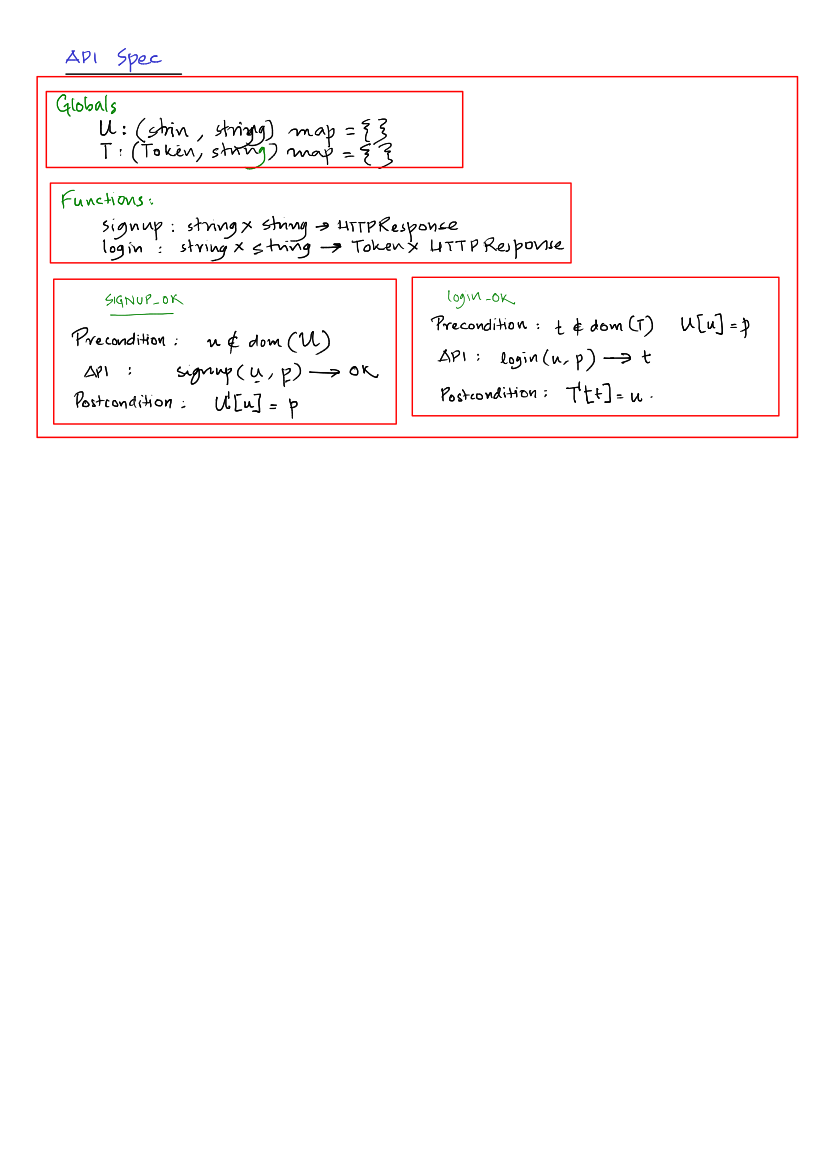
\includegraphics[width=\textwidth]{../images/spec-AST-1.png}
\end{center}
\caption{Example: API specification}
\label{f:spec}
\end{figure}

\subsubsection{Abstract Syntax Tree}
\begin{center}
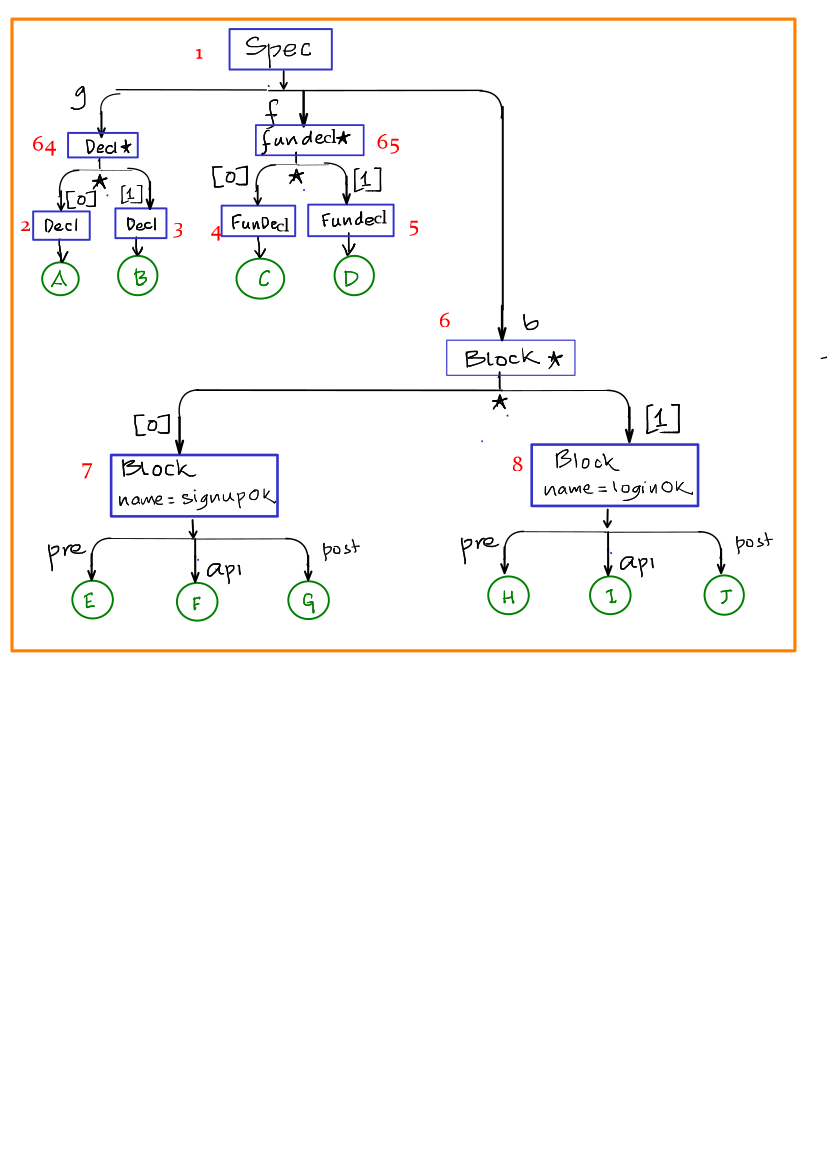
\includegraphics[width=\textwidth]{../images/spec-AST-2.png}

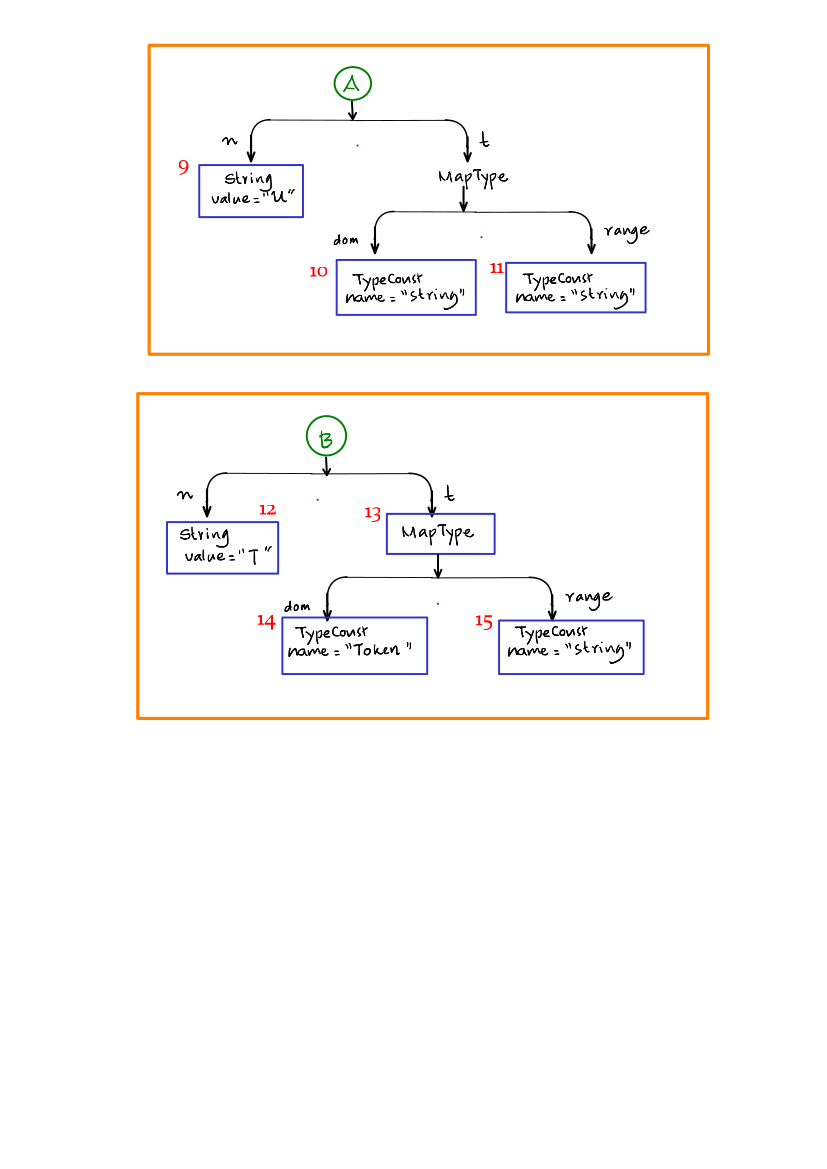
\includegraphics[width=\textwidth]{../images/spec-AST-3.png}

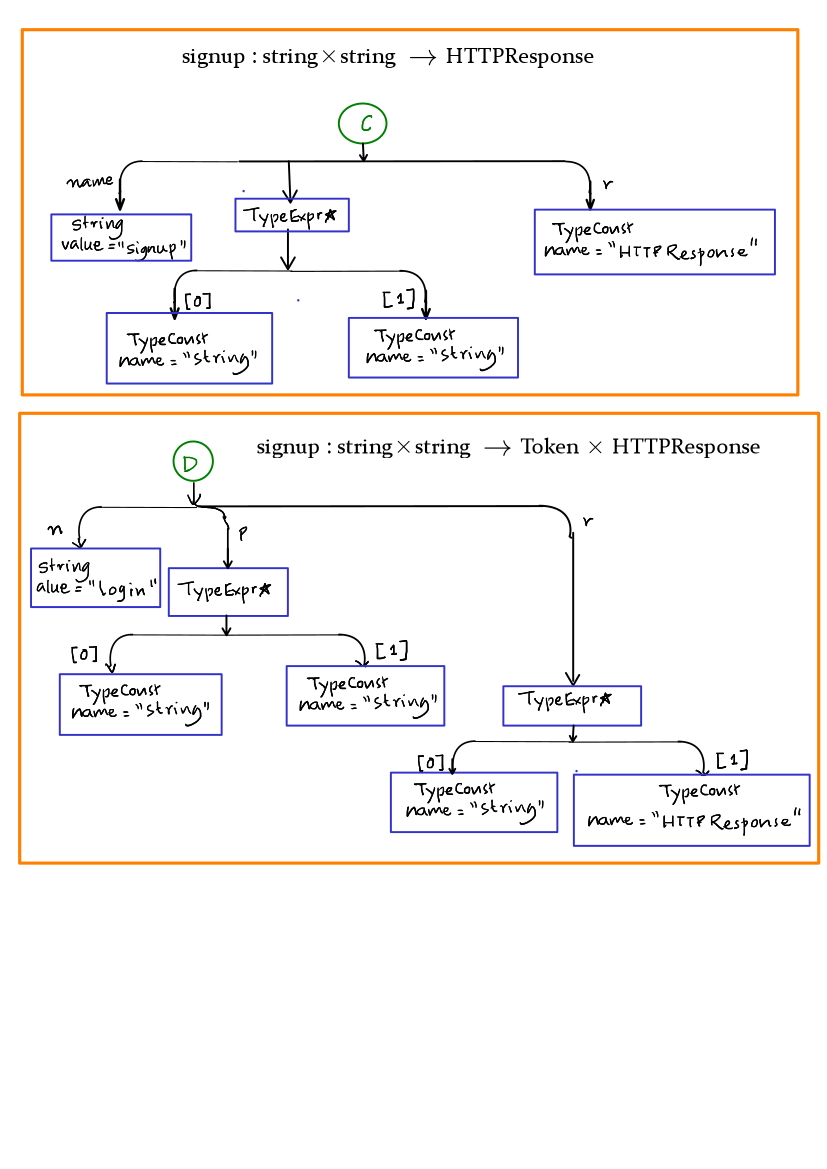
\includegraphics[width=\textwidth]{../images/spec-AST-4.png}

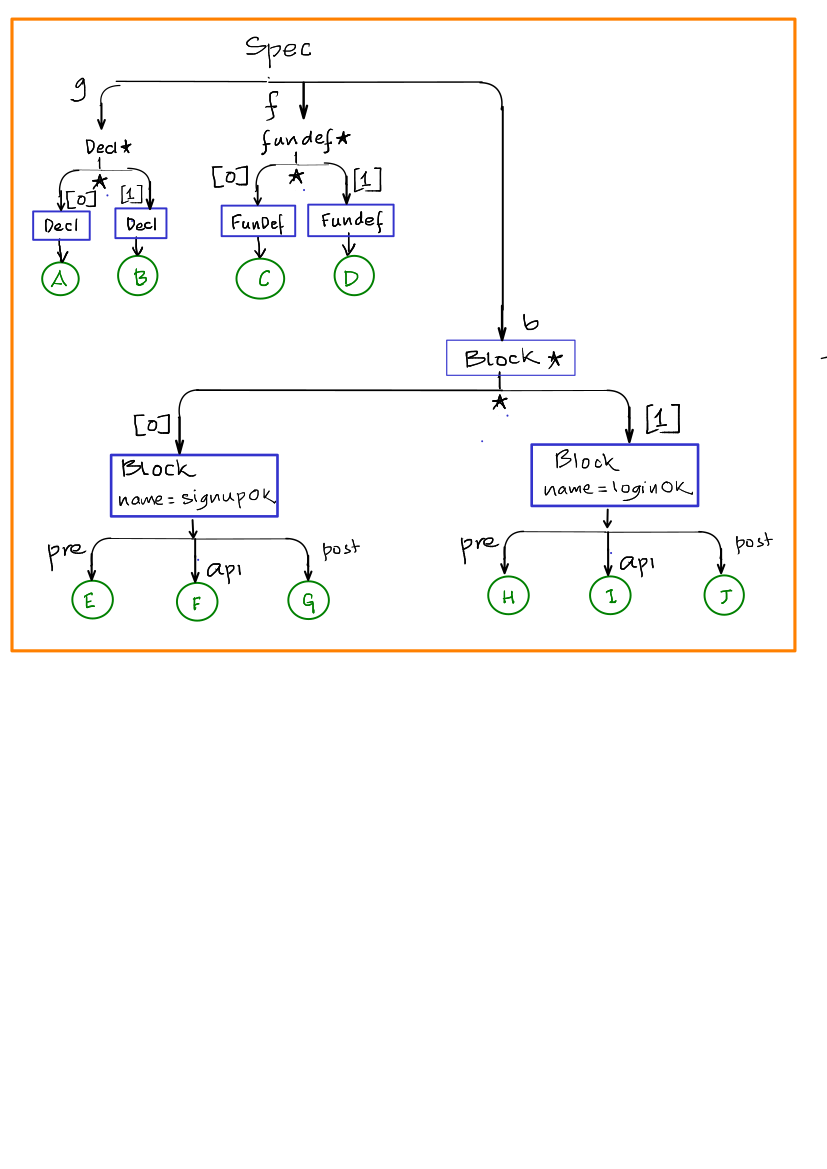
\includegraphics[width=\textwidth]{../images/spec-AST-5.png}

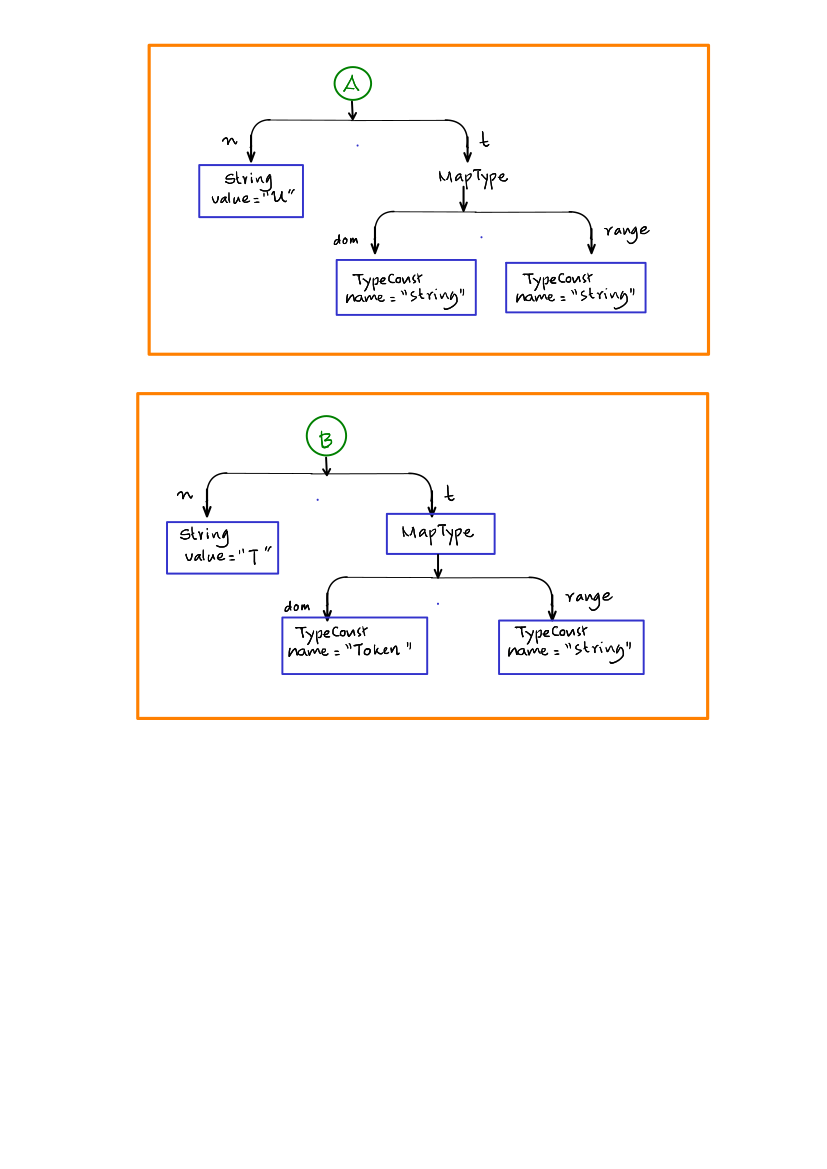
\includegraphics[width=\textwidth]{../images/spec-AST-6.png}

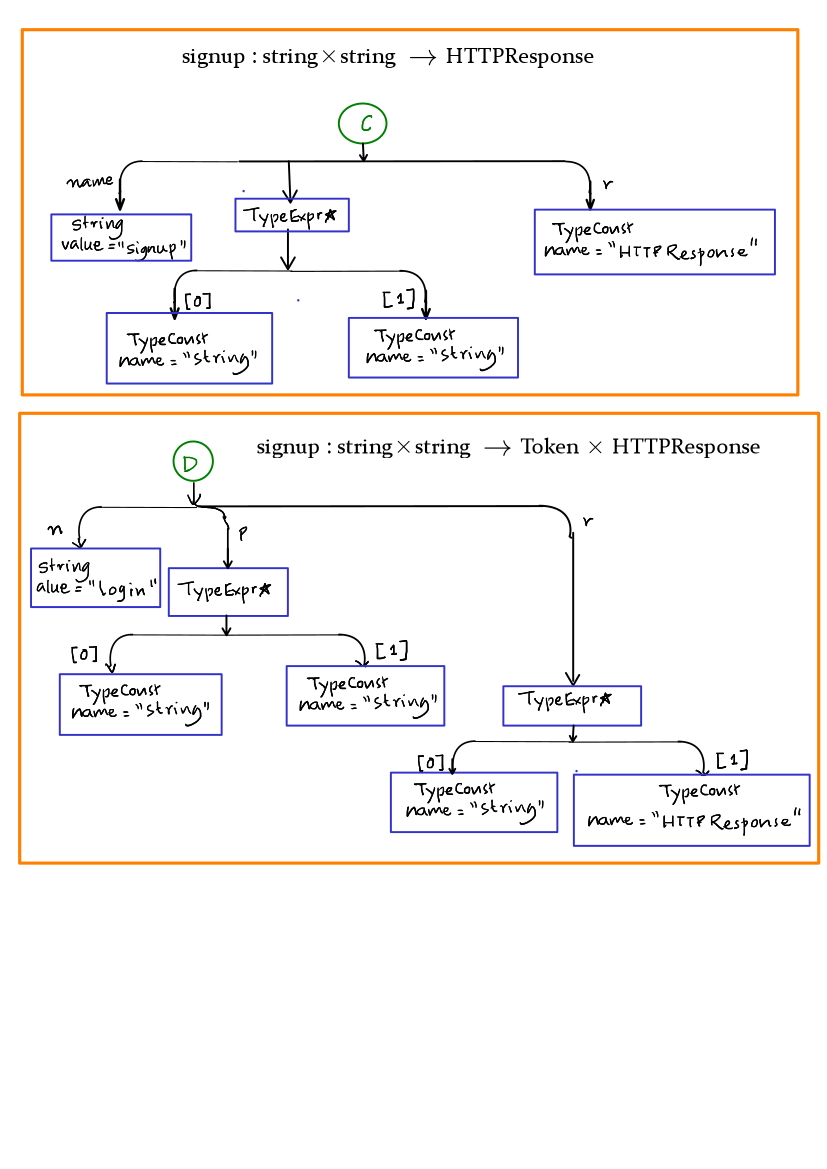
\includegraphics[width=\textwidth]{../images/spec-AST-7.png}

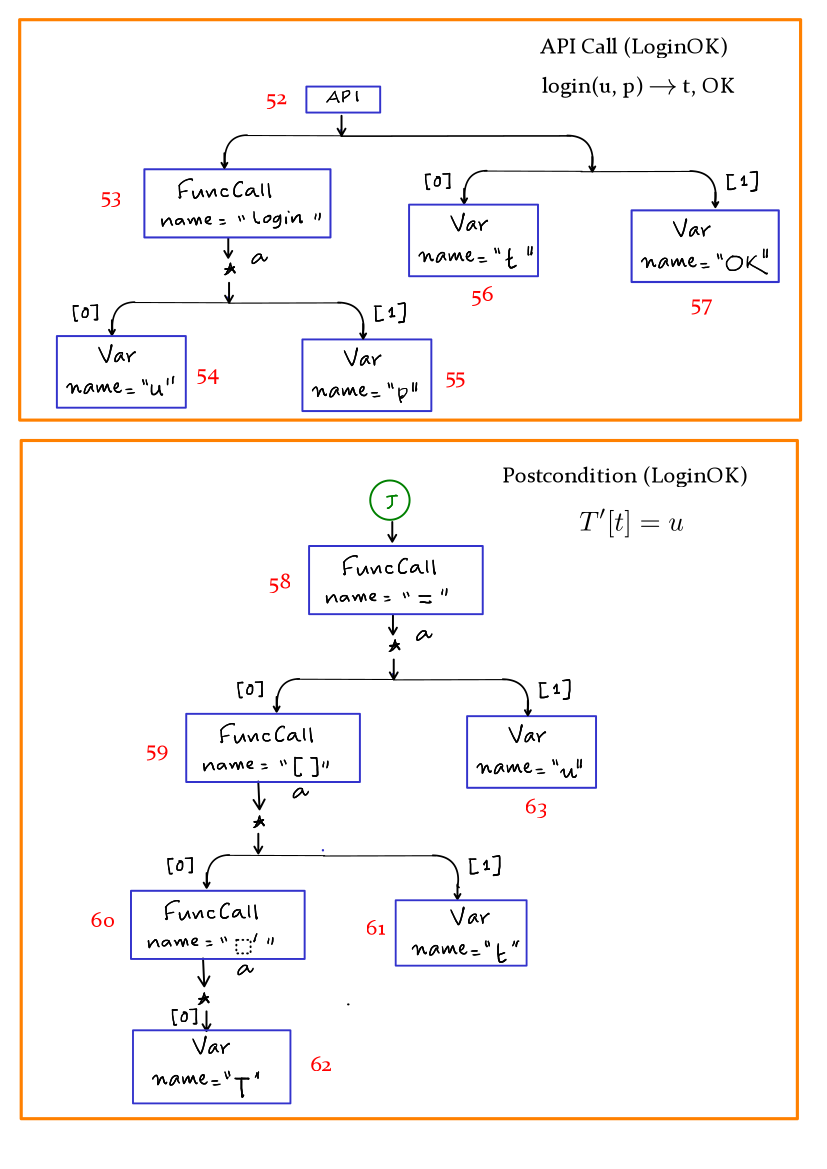
\includegraphics[width=\textwidth]{../images/spec-AST-8.png}
\end{center}

\section{Abstract Test Case}
\subsection{Abstract Syntax}
\begin{figure}
\begin{tabular}{l @{\hspace{1cm}} c @{\hspace{1cm}} p{10cm}}
\hline
$Program$ & \myprod & ($s$ : $Stmt\mathtt{*}$) \\
           & \mychoice & ({\color{Magenta} More will be added as we get more examples}) \\
$Stmt$ & \myprod & $Assign$ \mychoice $FuncCallStmt$ \\
$Assign$ & \myprod & ($l$ : $Var$, $r$ : $Expr$) \\
$FuncCallStmt$ & \myprod & ($f$ : $FuncCall$) \\
\hline
\end{tabular}
\caption{Abstract Syntax: Abstract Test Cases}
\label{f:syntax-act}
\end{figure}

\subsection{Example Abstract Test Case -- Signup(OK)$\rightarrow$Login(OK)}
\begin{figure}

\begin{center}
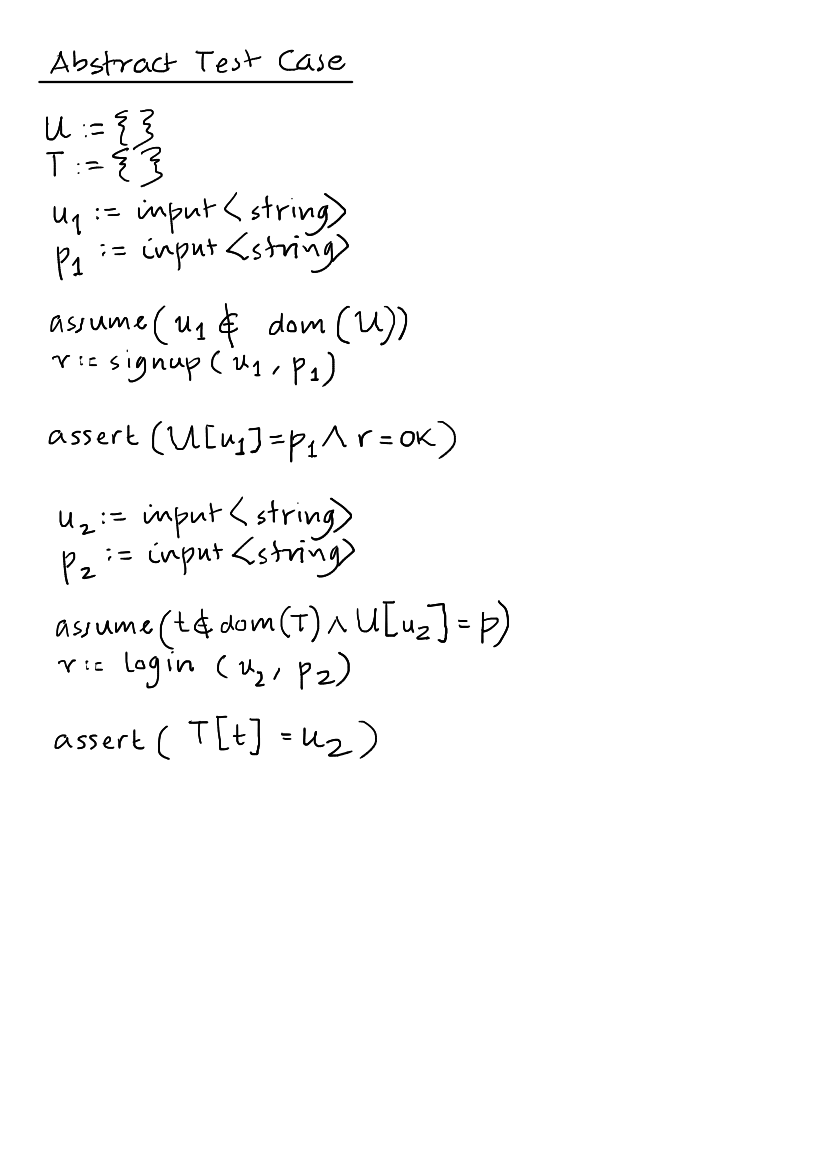
\includegraphics[width=\textwidth]{../images/spec-AST-9.png}
\end{center}
\caption{Example -- Abstract test case}
\label{f:act}
\end{figure}

\subsubsection{Abstract Syntax Tree}
\begin{center}
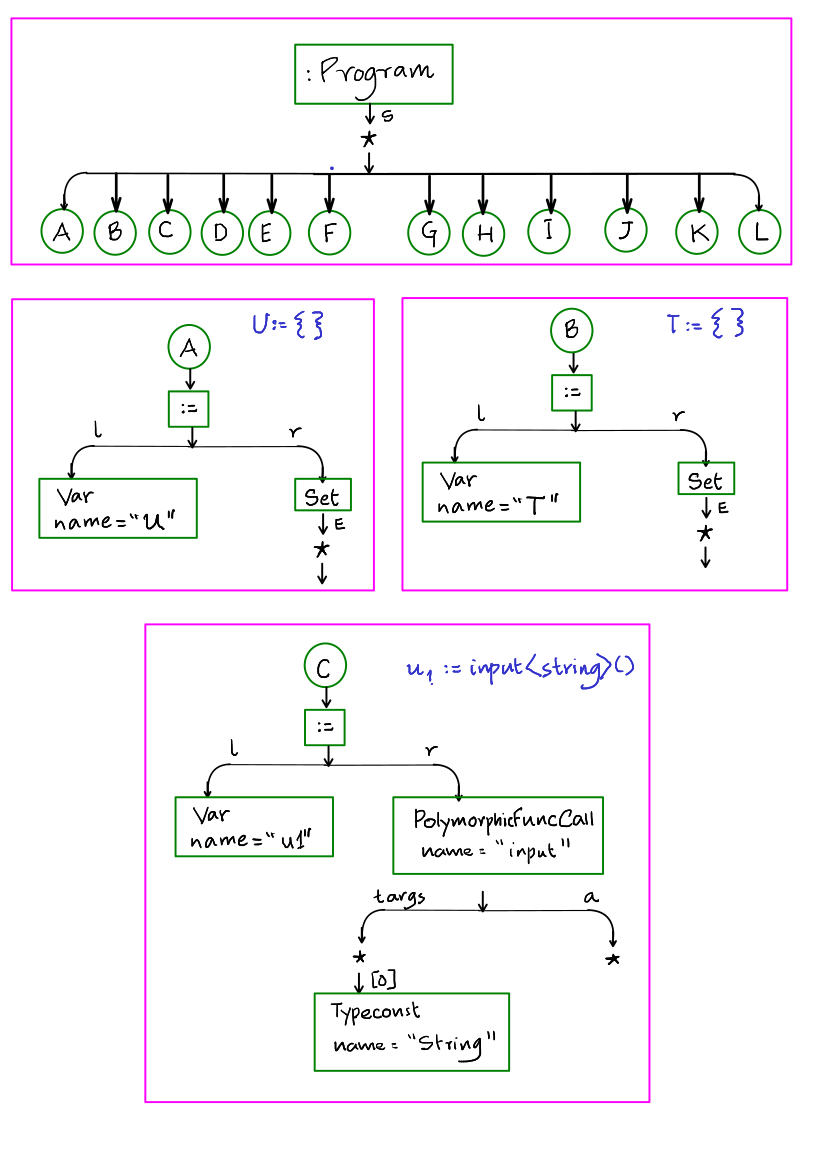
\includegraphics[width=\textwidth]{../images/ACT-AST-10.png}

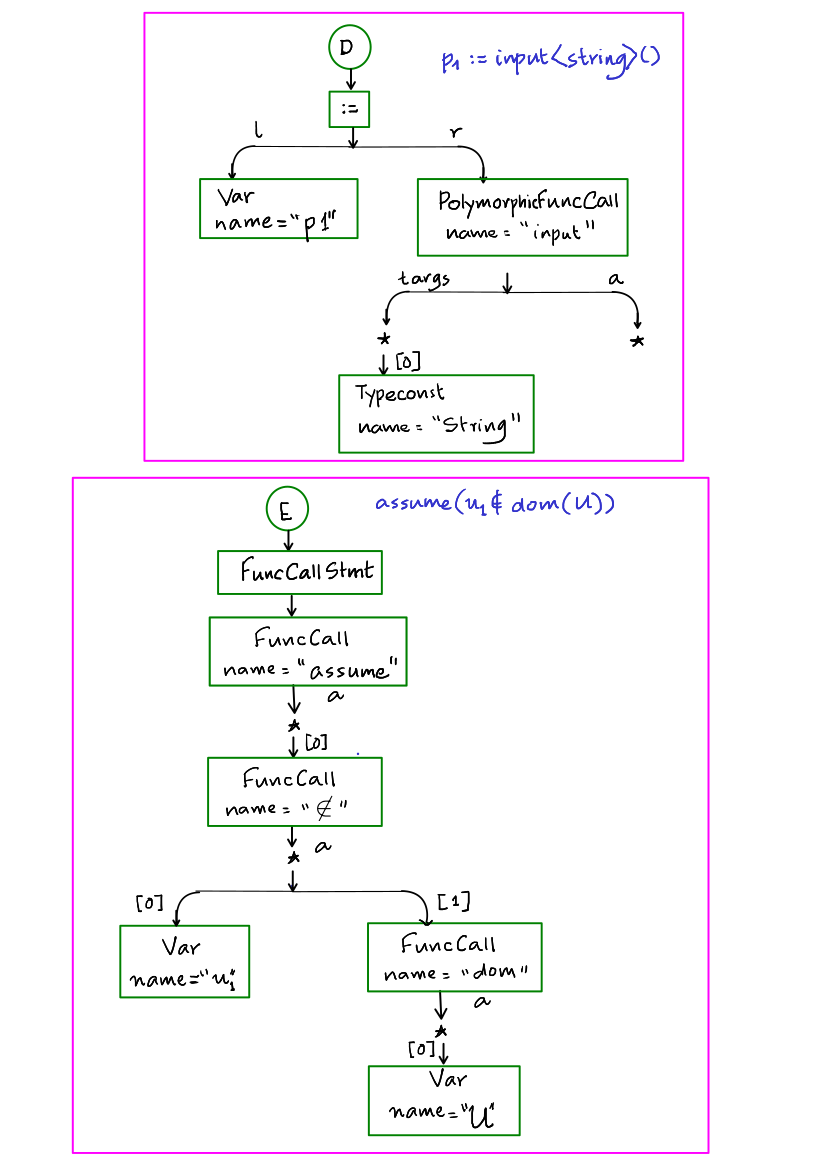
\includegraphics[width=\textwidth]{../images/ACT-AST-11.png}

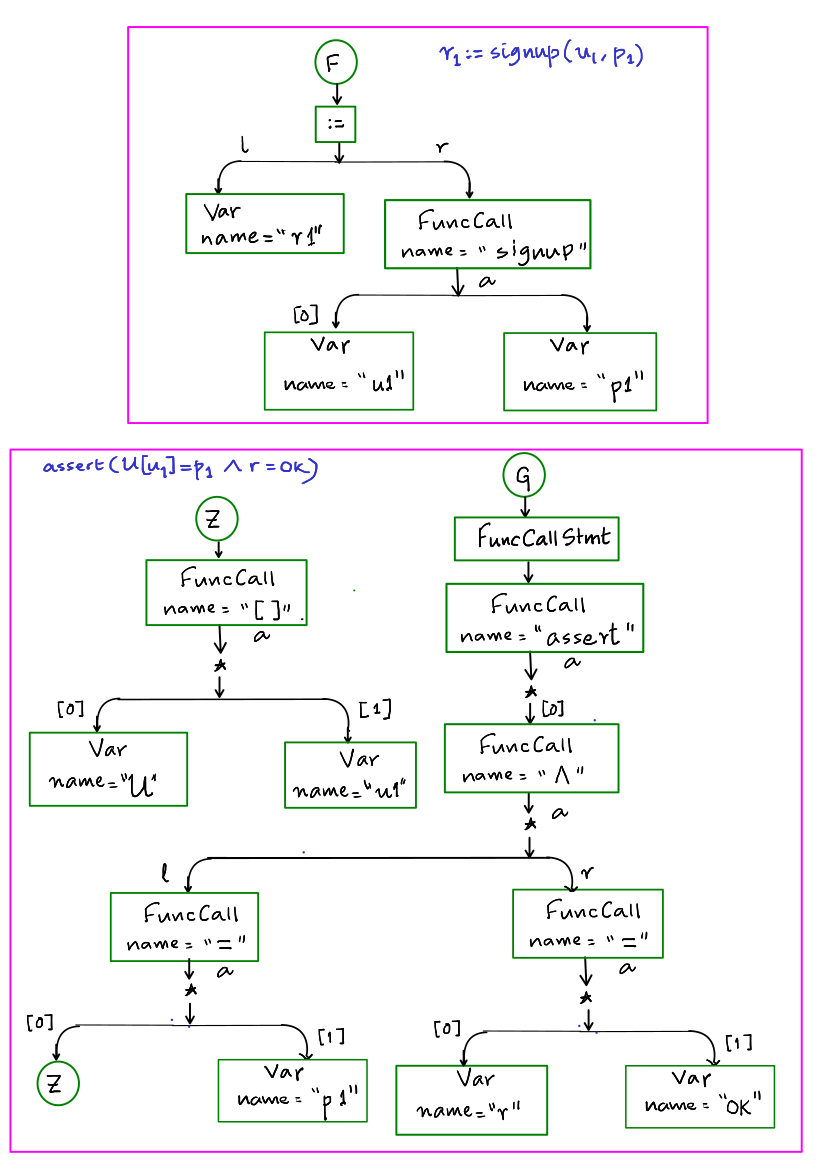
\includegraphics[width=\textwidth]{../images/ACT-AST-12.png}

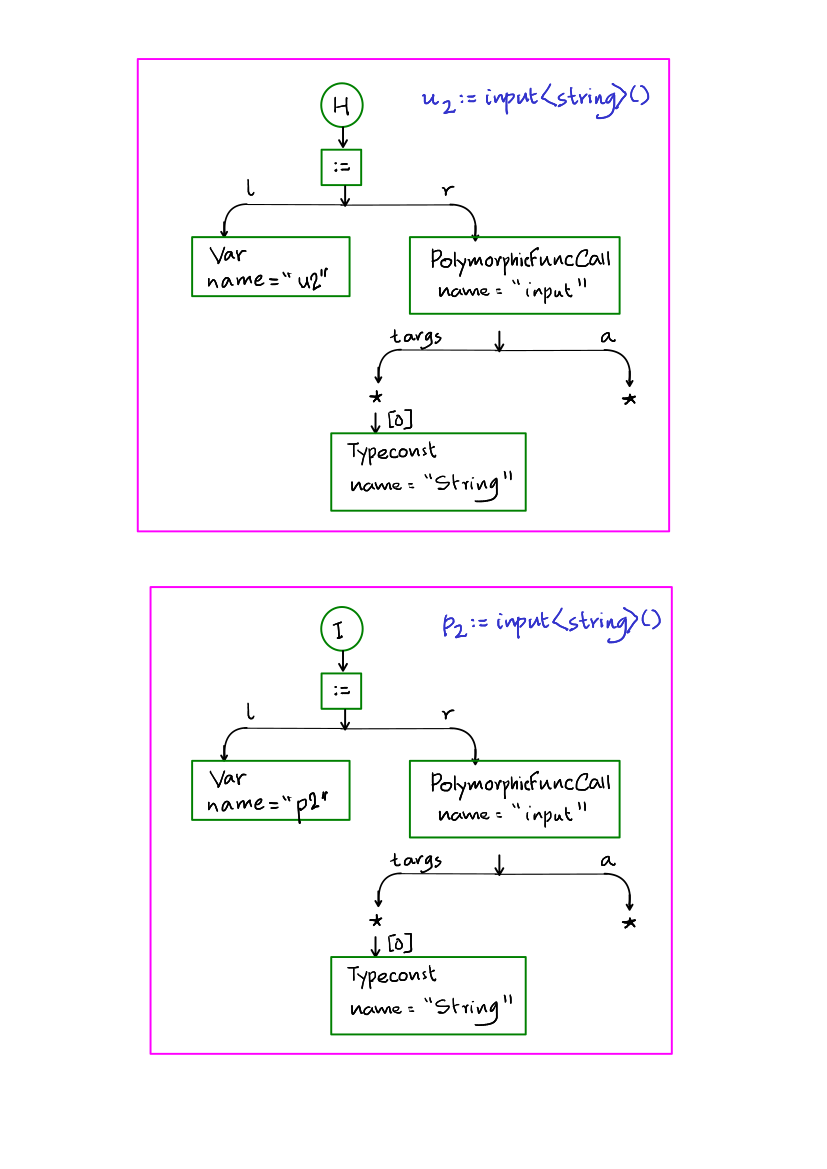
\includegraphics[width=\textwidth]{../images/ACT-AST-13.png}

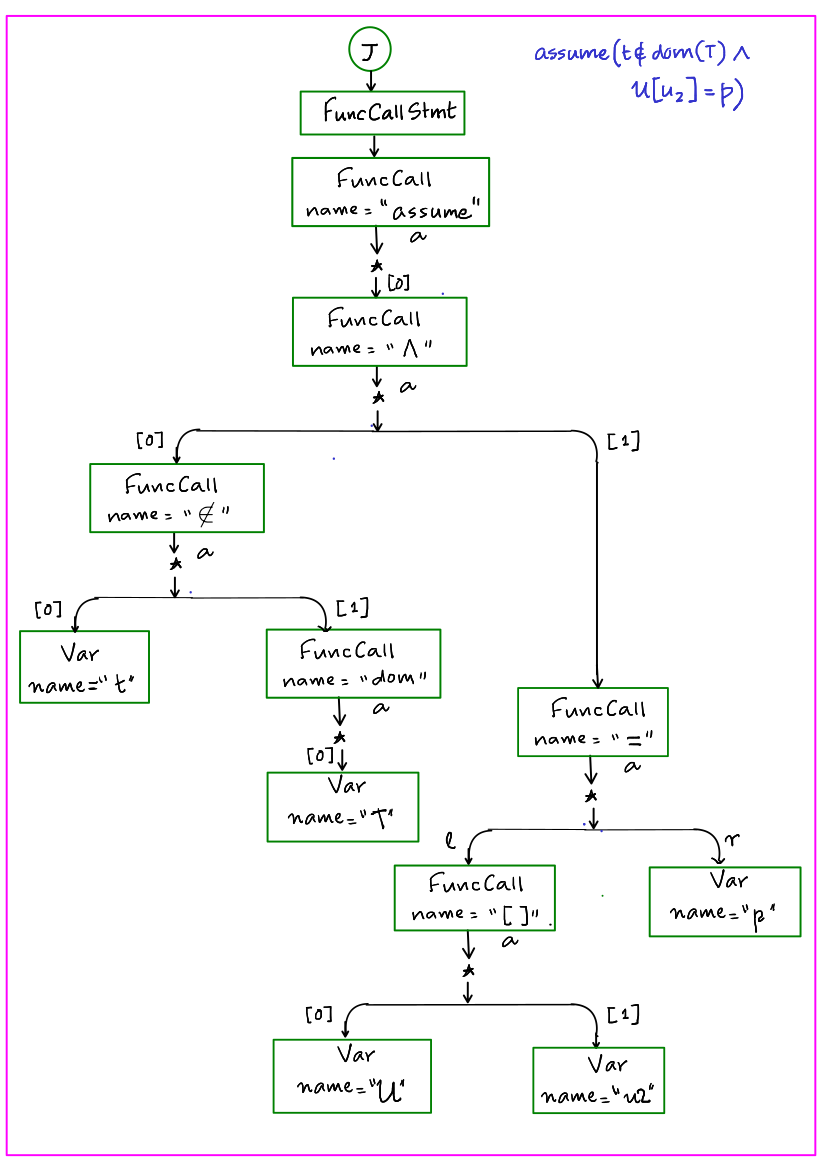
\includegraphics[width=\textwidth]{../images/ACT-AST-14.png}

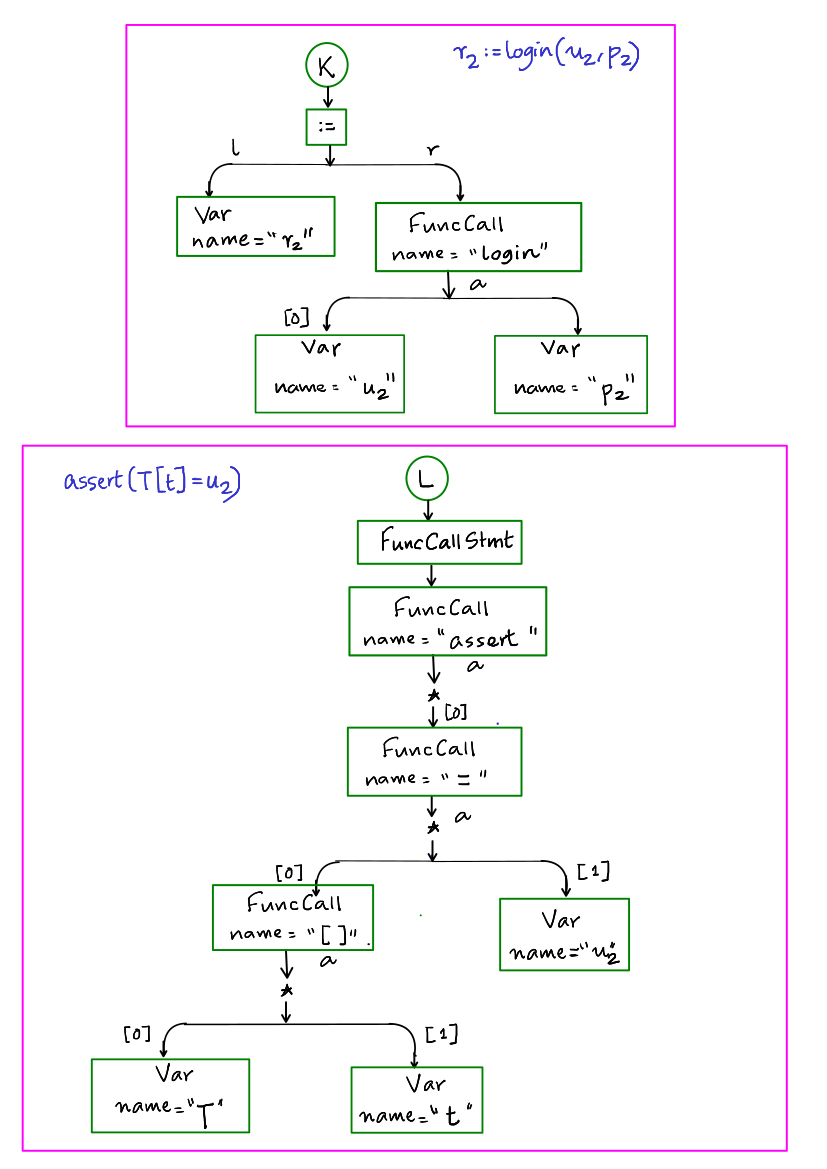
\includegraphics[width=\textwidth]{../images/ACT-AST-15.png}
\end{center}
\end{document}
